%======================================================================
\chapter{Light and Focusing }
\label{Ch:LightAndFocusing}
%======================================================================
\textbf{This chapter is based on the following manuscript:}
\begin{enumerate}
    \item \textbf{Author 1}, Author 2, Supervisor 1, ``Theoretical analysis of light and focus", \textit{Optics Expresso} \textbf{28}, 20026-20028 (2026) 
    DOI: \href{https://doi.org/10.1364/OE.395054}{https://doi.org/}
\end{enumerate}

In the past decades, the use of structured light has revolutionized the field of light and structures. In this chapter, we present a detailed theoretical analysis ... . The formalism used to describe focusing is discussed ~\ref{sec:Focusedfields}. The numerical implementation used in this work can be found in Appendix \ref{AppendixA}. We believe the results can be used for something.


%======================================================================
\section{Focused Fields}
\label{sec:Focusedfields}
%======================================================================

There was a light beam and it got focused! The experimental implementation is shown in \ref{fig:TF}
\begin{figure}[H]
    \centering
    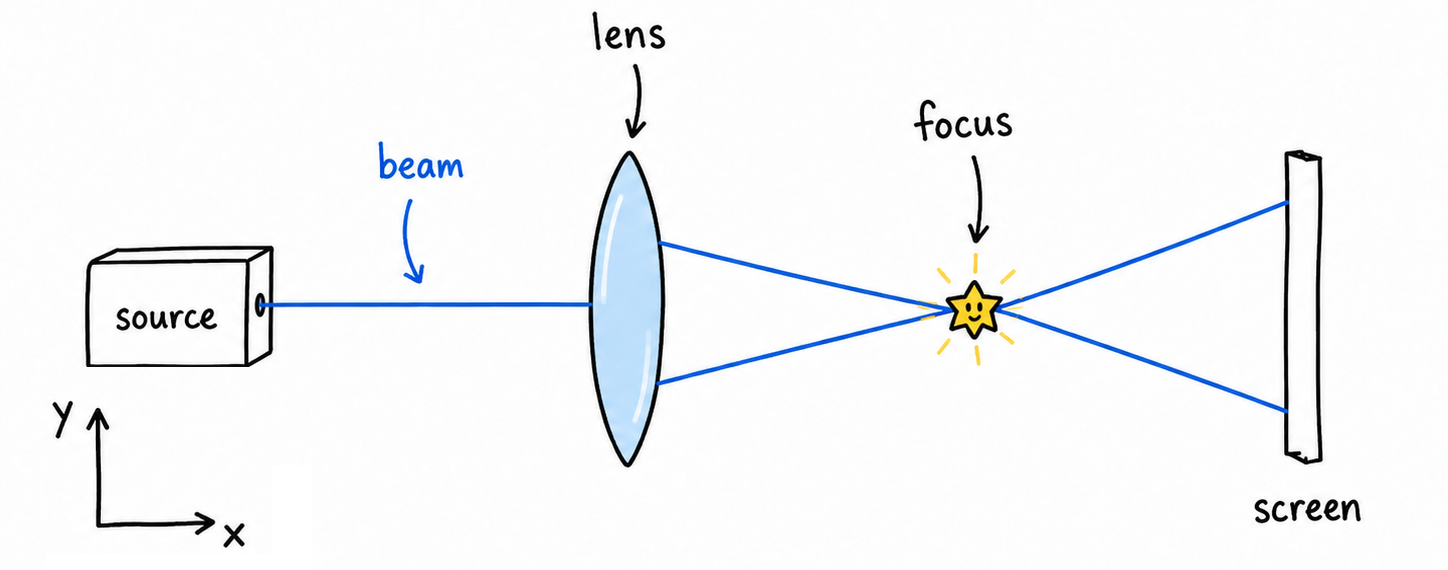
\includegraphics[width=0.9\textwidth]{figures/C2/fig-focusing.png}
    \caption{ \textbf{Focusing of optical beams: a.} Schematic diagram  of the focusing of light}
    \label{fig:TF}
\end{figure}



 \Publication{\textbf{Publication: }Focusing is awesome
}{PDF/DummyArticle}


